\section{peo\-Seq\-Pop\-Eval$<$ EOT $>$ Class Template Reference}
\label{classpeo_seq_pop_eval}\index{peoSeqPopEval@{peoSeqPopEval}}
The {\bf peo\-Seq\-Pop\-Eval}{\rm (p.\,\pageref{classpeo_seq_pop_eval})} class acts only as a Paradis\-EO specific sequential evaluation functor - a wrapper for incorporating an {\bf eo\-Eval\-Func$<$ EOT $>$}-derived class as evaluation functor.  


{\tt \#include $<$peo\-Seq\-Pop\-Eval.h$>$}

Inheritance diagram for peo\-Seq\-Pop\-Eval$<$ EOT $>$::\begin{figure}[H]
\begin{center}
\leavevmode
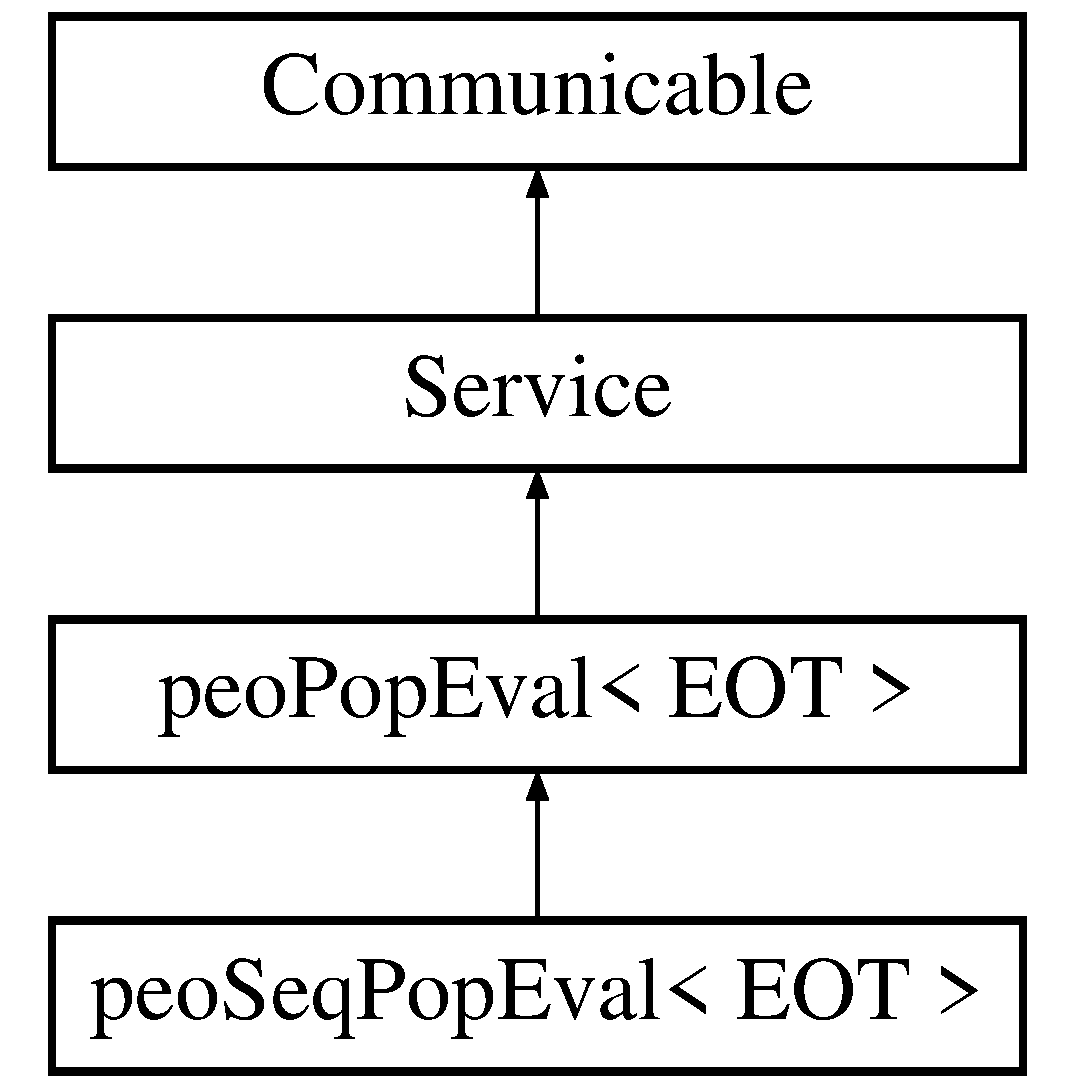
\includegraphics[height=4cm]{classpeo_seq_pop_eval}
\end{center}
\end{figure}
\subsection*{Public Member Functions}
\begin{CompactItemize}
\item 
{\bf peo\-Seq\-Pop\-Eval} (eo\-Eval\-Func$<$ EOT $>$ \&\_\-\_\-eval)
\begin{CompactList}\small\item\em Constructor function - it only sets an internal reference to point to the specified evaluation object. \item\end{CompactList}\item 
void {\bf operator()} (eo\-Pop$<$ EOT $>$ \&\_\-\_\-pop)
\begin{CompactList}\small\item\em Operator for evaluating all the individuals of a given population - in a sequential iterative manner. \item\end{CompactList}\end{CompactItemize}
\subsection*{Private Attributes}
\begin{CompactItemize}
\item 
eo\-Eval\-Func$<$ EOT $>$ \& {\bf eval}\label{classpeo_seq_pop_eval_5465f31386c6b96bc8f7fb9393a28a2f}

\end{CompactItemize}


\subsection{Detailed Description}
\subsubsection*{template$<$class EOT$>$ class peo\-Seq\-Pop\-Eval$<$ EOT $>$}

The {\bf peo\-Seq\-Pop\-Eval}{\rm (p.\,\pageref{classpeo_seq_pop_eval})} class acts only as a Paradis\-EO specific sequential evaluation functor - a wrapper for incorporating an {\bf eo\-Eval\-Func$<$ EOT $>$}-derived class as evaluation functor. 

The specified EO evaluation object is applyied in an iterative manner to each individual of a specified population. 



Definition at line 36 of file peo\-Seq\-Pop\-Eval.h.

\subsection{Constructor \& Destructor Documentation}
\index{peoSeqPopEval@{peo\-Seq\-Pop\-Eval}!peoSeqPopEval@{peoSeqPopEval}}
\index{peoSeqPopEval@{peoSeqPopEval}!peoSeqPopEval@{peo\-Seq\-Pop\-Eval}}
\subsubsection{\setlength{\rightskip}{0pt plus 5cm}template$<$class EOT$>$ {\bf peo\-Seq\-Pop\-Eval}$<$ EOT $>$::{\bf peo\-Seq\-Pop\-Eval} (eo\-Eval\-Func$<$ EOT $>$ \& {\em \_\-\_\-eval})}\label{classpeo_seq_pop_eval_a41f91ab4b2aeb325ff75feb66d4e003}


Constructor function - it only sets an internal reference to point to the specified evaluation object. 

\begin{Desc}
\item[Parameters:]
\begin{description}
\item[{\em eo\-Eval\-Func$<$}]EOT $>$\& \_\-\_\-eval - evaluation object to be applied for each individual of a specified population \end{description}
\end{Desc}


Definition at line 56 of file peo\-Seq\-Pop\-Eval.h.

\subsection{Member Function Documentation}
\index{peoSeqPopEval@{peo\-Seq\-Pop\-Eval}!operator()@{operator()}}
\index{operator()@{operator()}!peoSeqPopEval@{peo\-Seq\-Pop\-Eval}}
\subsubsection{\setlength{\rightskip}{0pt plus 5cm}template$<$class EOT$>$ void {\bf peo\-Seq\-Pop\-Eval}$<$ EOT $>$::operator() (eo\-Pop$<$ EOT $>$ \& {\em \_\-\_\-pop})\hspace{0.3cm}{\tt  [virtual]}}\label{classpeo_seq_pop_eval_b2c88b9a3ad9091949acf741844eb02f}


Operator for evaluating all the individuals of a given population - in a sequential iterative manner. 

\begin{Desc}
\item[Parameters:]
\begin{description}
\item[{\em eo\-Pop$<$}]EOT $>$\& \_\-\_\-pop - population to be evaluated. \end{description}
\end{Desc}


Implements {\bf peo\-Pop\-Eval$<$ EOT $>$} {\rm (p.\,\pageref{classpeo_pop_eval_2f208067a5e39c3b26c1234050a41e8f})}.

Definition at line 61 of file peo\-Seq\-Pop\-Eval.h.

References peo\-Seq\-Pop\-Eval$<$ EOT $>$::eval.

The documentation for this class was generated from the following file:\begin{CompactItemize}
\item 
peo\-Seq\-Pop\-Eval.h\end{CompactItemize}
